 
\usepackage[round]{natbib}
\usepackage{tikz} 
\usepackage{mathptmx}
\usepackage[T1]{fontenc}
\usepackage[latin1]{inputenc}
\usepackage{color}
\usepackage{amsmath}
\usepackage{amssymb}

\only<beamer|trans|handout|draft>{
\newcommand{\newblock}{}
}

\usepackage{listings}
%%%%%%%%%% Farseerfc: fix the bug of xetex on navigation bar of beamer %%%%%%%%%

\def\beamer@linkspace#1{%
  \begin{pgfpicture}{0pt}{-1.5pt}{#1}{5.5pt}
    \pgfsetfillopacity{0}
    \pgftext[x=0pt,y=-1.5pt]{.}
    \pgftext[x=#1,y=5.5pt]{.}
  \end{pgfpicture}}

%%%%%%%%%% Farseerfc: fix the bug of xetex on navigation bar of beamer %%%%%%%%%

\usetheme{Warsaw}
\usecolortheme[named=OliveGreen]{structure}
%\setbeamercovered{dynamic}
\useoutertheme{infolines}
\usepackage[english]{babel}


\graphicspath{{figure/}}
\begin{document}

%%%%%%%%%%%%%%%%%%%%%%%%%%%%%%%%%%%%%%%%%%%%%%%%%%%%%%%%%%%%%%%%%%%%%%%%%%%%%%%%
% Farseerfc defined commands

\newcommand{\br}[0]{\par\vskip15pt\par}
%\newenvironment{topcolumns}{\begin{columns}[t]}{\end{columns}}

%%%%%%%%%%%%%%%%%%%%%%%%%%%%%%%%%%%%%%%%%%%%%%%%%%%%%%%%%%%%%%%%%%%%%%%%%%%%%%%%



\title[report]{Report of Progress}


\subtitle{by Jiachen Yang}

\author[jc-yang]{
	Jiachen Yang\inst{1} 
}

\institute[Osaka-U]{
	\inst{1}Research Student in Osaka University
}



\frame{\maketitle}


\AtBeginSubsection[]{
  \frame<beamer>{ 
    \frametitle{Section Outline}   
    \tableofcontents[currentsection,currentsubsection] 
  }
}

\AtBeginSection[]{
  \frame<beamer>{ 
    \frametitle{Part Outline}   
    \tableofcontents[currentpart,currentsection] 
  }
}

\AtBeginPart{
  \frame<beamer>{
	\partpage
  }
}

%%%%%%%%%%%%%%%%%%%%%%%%%%%%%%%%%%%%%%%%%%%%%%%%%%%%%%%%%%%%%%%%%%%%%%%%%%%%%%%%
\section{In last week} 

\begin{frame}{Works in last week}

\begin{itemize}
\item Implemented Generalized Suffix Tree to extract 
Maximal Common Sequence from multiple input files.
\item Changed tokeinze framework from "tokenize" package in Python to
PLY(Python Lex-Yacc) project.

Add other language support in future.
\end{itemize}

Paper reading \cite{roy2007survey}, \cite{rainer2008using},
      \cite{smith2009detecting}.

\bibliographystyle{abbrvnat}
\bibliography{ref}
\end{frame}

%%%%%%%%%%%%%%%%%%%%%%%%%%%%%%%%%%%%%%%%%%%%%%%%%%%%%%%%%%%%%%%%%%%%%%

\begin{frame}{Generalized Suffix Tree}

\transfade
What is GST


\begin{itemize}
\item Generalized Suffix Tree(GST): 
    A Suffix Tree that contains multiple strings.

\item Adventage: Find Maximal Common Sequence(MCS) in linear time of 
sum of length of strings.
\item Disadvantage: All strings are stored in memory.
\end{itemize}

\pause
Building GST:
\begin{enumerate}
\item Append each string with a unique terminal mark(\$)
\item Concat strings as a long string. 

STRING1\alert{$\$_1$}STRING2\alert{$\$_2$}STRING3\alert{$\$_3$}...
\item build normal Suffix Tree with this long string
\item find CS that terminate at different terminal marks.
\end{enumerate}

\end{frame}

\begin{frame}[fragile]{GST example}%

\begin{figure}
\caption{Suffix Tree of abcd\_dbca\#}
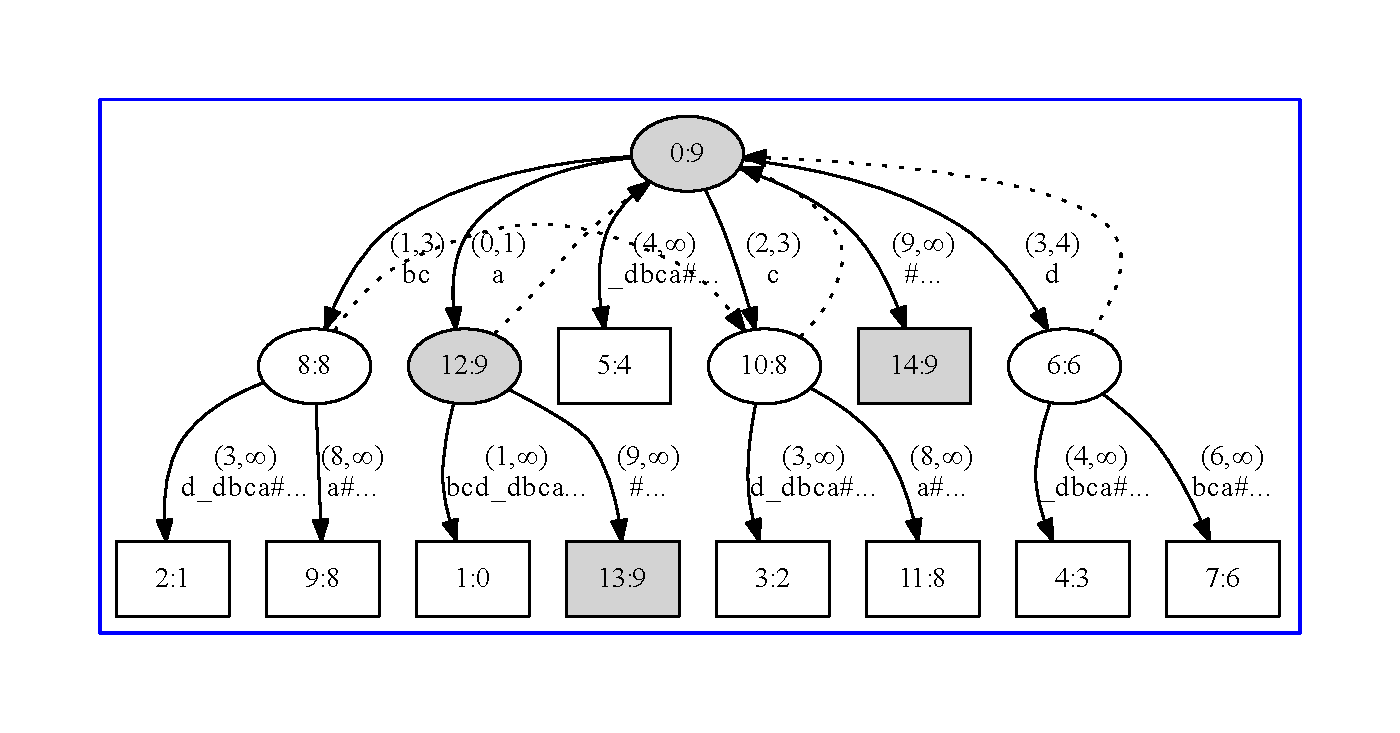
\includegraphics[width=0.8\textwidth,trim=40pt 40pt 40pt 40pt]{gst.pdf}
\end{figure}

\begin{lstlisting}
$ echo abcd_dbca# | ../filter.py
bc	2:{1, 6}
\end{lstlisting}

\end{frame}

\begin{frame}{Implement GST on multiple token sequence}
\begin{enumerate}
\item Append each token sequence with a unique ENDMARK.
\item Build a list with positions of ENDMARKs.

ENDMARK list looks like: \{100,300,500,800\}
\item A filter on generated MCS that 
\begin{itemize}
\item compare MCS end index with ENDMARK list.

MCS looks like: 40, \{120,330,600\}

end-index of above MCS is: \{160,370,640\}
\item extract those MCS that ends at different ENDMARK position.
\end{itemize}
\end{enumerate}

This approach can extract MCS in different \alert{files} as well as 
in different \alert{groups of files}.
\end{frame}


\begin{frame}[fragile,shrink=10]{Example of GST filter on python token sequence}
\lstset{breaklines=true}
\begin{lstlisting}
$ ./st_token.py *.py
62:{7213, 8150}	NAME,NEWLINE,DEDENT,DEDENT,CLASS,NAME,COLON,NEWLINE,INDENT,DEF,NAME,LPAR,NAME,COMMA,NAME,COMMA,NAME,COMMA,NAME,COMMA,NAME,RPAR,COLON,NEWLINE,INDENT,NAME,DOT,NAME,EQUAL,NAME,NEWLINE,NAME,DOT,NAME,EQUAL,NAME,NEWLINE,NAME,DOT,NAME,EQUAL,NAME,NEWLINE,NAME,DOT,NAME,EQUAL,NAME,NEWLINE,DEDENT,DEF,NAME,LPAR,NAME,RPAR,COLON,NEWLINE,INDENT,RETURN,NAME,DOT,NAME
60:{304, 6196}	COMMA,STRING,COMMA,STRING,COMMA,STRING,COMMA,STRING,COMMA,STRING,COMMA,STRING,COMMA,STRING,COMMA,STRING,COMMA,STRING,COMMA,STRING,COMMA,STRING,COMMA,STRING,COMMA,STRING,COMMA,STRING,COMMA,STRING,COMMA,STRING,COMMA,STRING,COMMA,STRING,COMMA,STRING,COMMA,STRING,COMMA,STRING,COMMA,STRING,COMMA,STRING,COMMA,STRING,COMMA,STRING,COMMA,STRING,COMMA,STRING,COMMA,STRING,COMMA,STRING,COMMA,STRING
40:{7997, 10214}	NAME,DOT,NAME,LSQB,NAME,RSQB,NEWLINE,DEDENT,DEF,NAME,LPAR,NAME,COMMA,NAME,COMMA,NAME,RPAR,COLON,NEWLINE,INDENT,NAME,DOT,NAME,LSQB,NAME,RSQB,EQUAL,NAME,NEWLINE,DEDENT,DEF,NAME,LPAR,NAME,COMMA,NAME,RPAR,COLON,NEWLINE,INDENT
\end{lstlisting}
\end{frame}

\begin{frame}{Experiment on GST} 
\alert{220} input files from Python 3.2 standard Library.

\alert{588,962} tokens.

in \alert{1m43.2s}

Cost \alert{644MiB} memory 

\end{frame}

\begin{frame}{Works in this week}
\begin{itemize}
\item Continue to read papers
\item Add c lexer support and other language support
\item idea of using n-gram to figure out "interesting" clones
\end{itemize}
\end{frame}

\end{document}
